\documentclass[conference]{IEEEtran}

\usepackage[T1]{fontenc}
\usepackage[utf8]{inputenc}
\usepackage{graphicx}
\usepackage{cite}
\usepackage{amsmath,amssymb}
\usepackage{booktabs}
\usepackage{tabularx}
\usepackage{array}
\usepackage{multirow}
\usepackage{enumitem}
\usepackage{float}
\usepackage{hyperref}
\usepackage{xcolor}
\usepackage{url}

\graphicspath{{./}}

\hypersetup{
  colorlinks=true,
  linkcolor=black,
  citecolor=black,
  urlcolor=blue
}

\newcolumntype{P}[1]{>{\raggedright\arraybackslash}p{#1}}
\newcolumntype{T}[1]{>{\scriptsize\raggedright\arraybackslash}p{#1}}

% ── Title ─────────────────────────────────────────────────────────────────────
\title{Intent-to-API Orchestration for Future Telco Networks:\\
A CAPIF-Aware, AI-Native Platform with Empirical\\
Reliability Evaluation}

\author{
\IEEEauthorblockN{T\"{u}rkan Do\u{g}a Durak}
\IEEEauthorblockA{
Centre Tecnol\`{o}gic de Telecomunicacions de Catalunya (CTTC)\\
Castelldefels, Spain\\
\texttt{turkandoga.durak@cttc.es}
}
}

\begin{document}
\maketitle

% ── Abstract ──────────────────────────────────────────────────────────────────
\begin{abstract}
Future Internet architectures demand programmable network exposure
frameworks that bridge high-level operator intents to concrete telecom API
invocations without manual payload composition. This paper presents
the design, implementation, and empirical evaluation of a cloud-native,
CAPIF-aware telco orchestration platform combining 3GPP CAPIF governance,
CAMARA-aligned service semantics, NEF-backed telecom realisation, and
LLM-assisted planning under a three-layer deterministic validator.
A two-phase schema-grounded planning pipeline separates service routing
from payload generation, eliminating payload-level LLM errors entirely.
Evaluation on a bilingual 60-entry ground-truth dataset using six formally
defined reliability metrics yields IWSR\,=\,100\,\% (deterministic) and
IWSR\,=\,95\,\% (LLM-assisted, Claude Haiku\,4.5), with perfect Schema
Compliance (SCR\,=\,100\,\%) and Semantic Validity (SVR\,=\,100\,\%)
in both modes and a Stability Score of SS\,=\,0.892.
A preliminary multi-provider comparison shows that the pluggable
multi-LLM dispatcher (Gemini\,2.5\,Flash, GPT-4o-mini, Claude Haiku\,4.5)
delivers consistent SCR\,=\,SVR\,=\,100\,\% across all providers,
confirming that the schema-grounding mechanism is provider-agnostic.
All LLM failures are Phase\,1 service-routing errors on deliberately
ambiguous intents; no payload schema violation occurs in either mode,
validating the effectiveness of schema-grounded Phase\,2 prompting.
The platform and evaluation dataset are publicly released as open-source
artefacts providing a reproducible baseline for intent-based orchestration
research.
\end{abstract}

\begin{IEEEkeywords}
intent-based networking, CAPIF, CAMARA, NEF, 5G/B5G service exposure,
LLM-assisted orchestration, reliability evaluation, zero-touch automation,
cloud-native, future internet
\end{IEEEkeywords}

% =============================================================================
\section{Introduction}
% =============================================================================

The emergence of Beyond-5G (B5G) and 6G network architectures elevates
programmable service exposure from an optional feature to a foundational
design principle of the Future Internet.
Standardised frameworks such as 3GPP CAPIF (TS\,23.222)~\cite{3gpp_capif}
and the CAMARA project~\cite{camara2022} define the governance, discovery,
and semantic layers enabling vertical industries to consume network
capabilities through well-defined APIs.
NEF-based provider stacks~\cite{nefsim2022} bridge those interfaces to the
underlying data plane, resolving identifiers, enforcing policies, and
returning structured monitoring results.

In this layered model, orchestration logic must translate natural-language
intents into precisely structured, multi-field API payloads that comply with
strict telecom domain constraints: E.164 phone formats, enumerated QoS
profiles, duration bounds, and live CAPIF registry membership.
Manual payload composition at this level is error-prone and scales poorly,
motivating automated intent-to-API translation.
Large language models (LLMs) offer a compelling approach~\cite{maatouk2025,flowmind2023};
however, telecom API payloads impose hard correctness constraints that
probabilistic generation cannot guarantee without external
enforcement~\cite{liu2024,telagentbench2025}.
Hallucinated service identifiers, malformed phone numbers, or invalid QoS
profile names would silently propagate to production networks if not
intercepted.

This paper addresses the gap between LLM planning capability and
telecom-grade reliability. The main contributions are:

\begin{itemize}[leftmargin=1.1em]
  \item a working, open-source CAPIF-aware telco orchestration platform
        operating against live CAMARA providers in a multi-container
        Docker deployment;
  \item a two-phase schema-grounded LLM planner with a pluggable
        multi-provider dispatcher (Gemini, OpenAI, Anthropic) and live
        CAPIF discovery injection;
  \item a three-layer deterministic validator (L1\,Pydantic schema,
        L2\,telecom semantic policy, L3\,CAPIF registry) with a bounded
        feedback correction loop that guarantees payload correctness
        independent of LLM quality;
  \item a bilingual 60-entry ground-truth evaluation dataset
        with difficulty stratification and multi-country phone coverage;
  \item six formally defined reliability metrics (IWSR, SCR, SVR, HR, SS,
        RRF) constituting a reusable evaluation framework for
        intent-to-API orchestration systems.
\end{itemize}

The remainder of the paper is organised as follows.
Section~\ref{sec:related} surveys related work.
Section~\ref{sec:arch} describes the platform architecture and deployment.
Section~\ref{sec:llm} details the LLM planning and validation layer.
Section~\ref{sec:eval} presents the evaluation framework and results.
Section~\ref{sec:discussion} discusses findings and limitations.
Section~\ref{sec:conclusion} concludes.

% =============================================================================
\section{Related Work}
\label{sec:related}
% =============================================================================

\subsection{Intent-Based Networking and Orchestration}

Intent-based networking (IBN) has been explored extensively at the NFV
orchestration level.
Rafiq et al.~\cite{rafiq2020} demonstrated deterministic
intent-to-descriptor translation across multiple orchestrators;
Saraiva de~Sousa et al.~\cite{saraiva2019} identified intent abstraction
as a key direction for adaptive service management;
and Coronado et al.~\cite{coronado2022} positioned intent-driven
closed-loop control as foundational to zero-touch 6G management.
These works operate at the orchestration lifecycle level and generally
assume structured intent inputs, not natural language.

\subsection{5G Network Exposure Infrastructure}

Molina~Sanchez et al.~\cite{molina2022} implemented CAPIF Core Function
as an open-source microservice (OpenCAPIF), enabling community
experimentation with 3GPP-compliant API exposure.
Fragkos et al.~\cite{nefsim2022} introduced NEFSim as an open NEF
experimentation platform covering the full 3GPP service exposure stack.
Turkovic et al.~\cite{turkovic2025} demonstrated 3GPP-compliant CAMARA
QoD and Location API integration in a real CAM testbed, measuring
end-to-end latency of 230--340\,ms.
Our work builds on these open platforms as provider components and
focuses on the intent translation and orchestration layer above them.

\subsection{LLMs for Telecom and Structured Output}

Maatouk et al.~\cite{maatouk2025} identified hallucination and output
inconsistency as primary risks for LLM deployment in telecom operations.
Liu et al.~\cite{liu2024} benchmarked structured-output compliance of
leading LLMs and found that GPT-4 achieves an average compliance score
of only 0.40 on JSON schema tasks.
Lee et al.~\cite{telagentbench2025} confirmed that multi-turn planning
tasks significantly degrade LLM pass rates in telecom agent scenarios.
Zeng et al.~\cite{flowmind2023} demonstrated near-perfect workflow
generation when LLMs are grounded in structured API descriptions,
the approach adopted in Phase\,2 of our planner.

\noindent\textbf{Research Gap.}
To the best of our knowledge, no prior work provides end-to-end empirical
reliability evaluation of LLM-based natural-language intent-to-API
translation within a live CAPIF-compliant 5G service exposure environment,
operating under simultaneous schema, semantic, and registry constraints,
and reporting a standardised six-metric reliability framework on a
bilingual ground-truth dataset.

% =============================================================================
\section{Platform Architecture}
\label{sec:arch}
% =============================================================================

\subsection{System Overview and Components}

The platform comprises nine functional components organised into four
logical tiers: a user-facing \emph{interface tier}, a
\emph{control-plane tier} containing orchestration logic, a
\emph{provider tier} hosting CAMARA API realisations, and a
\emph{persistence tier} backed by MongoDB.
Fig.~\ref{fig:arch} depicts the complete cloud-native deployment topology;
Table~\ref{tab:components} summarises each component's responsibility.

\begin{table}[t]
\caption{Implemented Platform Components}
\label{tab:components}
\centering
\small
\begin{tabularx}{\linewidth}{P{0.30\linewidth} X}
\toprule
\textbf{Component} & \textbf{Responsibility} \\
\midrule
Operator Interface    & Product-style landing page with embedded OpenAPI console \\
FastAPI Backend       & Route handling, orchestration, validation, execution \\
Intent Engine         & Deterministic keyword-based routing (baseline mode) \\
LLM Planner           & Two-phase schema-grounded structured planning \\
Multi-Layer Validator & L1 Pydantic schema, L2 semantic policy, L3 CAPIF registry \\
Feedback Engine       & Bounded correction loop (max 3 iterations) \\
CAPIF Client          & Invoker onboarding, mTLS discovery, provider publication \\
Provider Layer        & QoD, Location Retrieval, QoS Provisioning, QoS Profiles \\
Persistence Layer     & MongoDB-backed NEF data with automatic initialisation \\
\bottomrule
\end{tabularx}
\end{table}

\begin{table}[t]
\caption{Main Backend Endpoints}
\label{tab:endpoints}
\centering
\small
\begin{tabularx}{\linewidth}{P{0.10\linewidth} T{0.36\linewidth} X}
\toprule
\textbf{Method} & \textbf{Path} & \textbf{Purpose} \\
\midrule
GET  & \path{/health}                 & Runtime health and mode summary \\
GET  & \path{/catalog/services}       & CAMARA-aligned capability catalog \\
POST & \path{/orchestrate}            & Intent-to-execution planning \\
GET  & \path{/capif/status}           & CAPIF connectivity check \\
POST & \path{/capif/invokers/onboard} & Live invoker onboarding \\
GET  & \path{/capif/discover}         & Live CAPIF service discovery \\
POST & \path{/capif/publish/catalog}  & Publish all catalog services \\
\bottomrule
\end{tabularx}
\end{table}

\begin{figure*}[t]
  \centering
  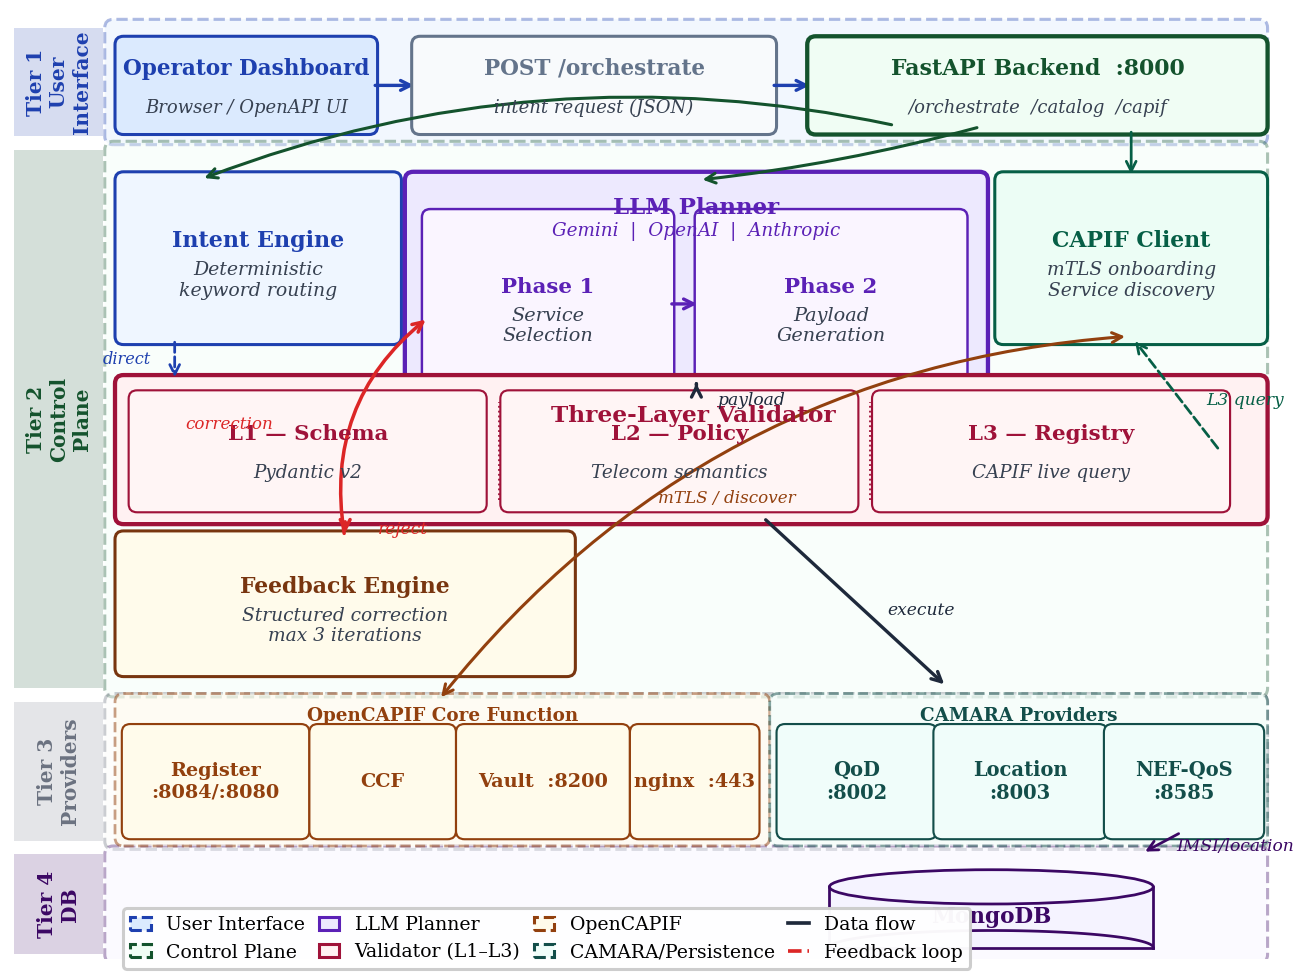
\includegraphics[width=0.96\textwidth]{nof_fig1_arch.png}
  \caption{Cloud-native system architecture of the Mini Telco Orchestration
  Platform. Tier\,1 (Operator Dashboard) submits intents via REST to
  Tier\,2 (Control Plane), where the FastAPI backend delegates to the
  Intent Engine (deterministic) or the two-phase LLM Planner.
  All payloads traverse a three-layer validator (L1--L3) with bounded
  feedback correction.
  Tier\,3a (OpenCAPIF Core Function at ports :8084/:8080 with Vault :8200
  and nginx :443) provides mTLS onboarding and live service discovery.
  Tier\,3b (CAMARA Providers at :8002, :8003, :8585) hosts QoD, Location
  Retrieval, and NEF-QoS.
  Tier\,4 (MongoDB) persists IMSI, location, and cell-polygon records;
  \texttt{mongo-init.js} seeds records on first deployment.
  All containers share the \texttt{capif-network} Docker bridge.}
  \label{fig:arch}
\end{figure*}

\subsection{Cloud-Native Multi-Container Deployment}

The platform is packaged as a Docker Compose stack comprising five
networked services: \textbf{backend} (FastAPI, port\,8000),
\textbf{OpenCAPIF Core Function} (3GPP-compliant register and discovery),
\textbf{NEF provider} (port\,8080), \textbf{camara-QoD provider}
(port\,8090), and \textbf{NEF-QoS provider} (port\,8585).
All containers share a Docker bridge network; service discovery across
providers is handled at runtime by the CAPIF client querying the Core
Function's discovery endpoint rather than through static configuration.
A named Docker volume persists MongoDB data across restarts, and an
initialisation script seeds location, IMSI, and polygon records on
first deployment.
The platform includes 65 automated unit tests across three pytest modules,
enabling CI/CD integration without any LLM API key or live CAPIF
connection as external dependencies.

\subsection{CAPIF Integration and CAMARA Service Realisation}

The backend acts as a CAPIF \textbf{Invoker}, following the 3GPP CAPIF-2e
reference point: (1)~authenticate against the register service;
(2)~generate an RSA private key and CSR locally;
(3)~submit the onboarding request to the CAPIF Core Function;
(4)~receive an \texttt{apiInvokerId} and certificate chain;
(5)~use mTLS for all subsequent discovery and execution.
CAMARA providers act as \textbf{API Exposing Functions (AEFs)},
publishing OpenAPI metadata through the CAPIF-4 reference point.
This three-role governance model ensures that every API invocation is
CAPIF-mediated: services are visible to the orchestration layer only
after publication, enabling the L3 validator to detect hallucinated
service identifiers via live registry queries.

The platform exposes four CAMARA-standardised orchestration targets:
\textit{QoD} for temporary QoS session creation (CAMARA QoD v1.1.0);
\textit{QoS Profiles} for available profile enumeration;
\textit{QoS Provisioning} for long-lived QoS assignment via 3GPP
AsSessionWithQoS (TS\,29.122); and \textit{Location Retrieval}
for device location access through NEF-backed MonitoringEvent
subscriptions (CAMARA Location-Retrieval v0.5).
The FRONT-research-group provider stacks~\cite{turkovic2025} are
included as Git submodules, enabling version-tracked integration.

% =============================================================================
\section{LLM-Assisted Orchestration}
\label{sec:llm}
% =============================================================================

\subsection{Two-Phase Schema-Grounded Planning}

The LLM planner implements a two-phase pipeline that separates service
routing from payload generation, limiting each call to a well-scoped
subtask with a clearly defined schema target (Fig.~\ref{fig:pipeline}).

\textit{Phase\,1 --- Service Selection:}
The LLM receives (a)~the user intent in natural language,
(b)~a schema-grounded summary of all CAMARA services extracted by
parsing YAML OpenAPI descriptors at startup, and (c)~optionally,
live CAPIF discovery results.
It returns a JSON object specifying \texttt{service\_id},
\texttt{operation\_id}, \texttt{method}, \texttt{path}, and a
\texttt{rationale} field for downstream traceability.

\textit{Phase\,2 --- Payload Generation:}
Given the Phase\,1 service selection, the LLM receives the full CAMARA
OpenAPI schema for that specific operation extracted at runtime.
It returns a complete, schema-aligned JSON payload matching the
operation's request body specification.
Grounding the payload prompt in the actual operation schema --- rather
than a generic description --- is the key mechanism achieving
SCR\,=\,100\,\% in LLM-assisted mode, confirming the FlowMind
hypothesis~\cite{flowmind2023} in a live telecom environment.

Three LLM providers are supported via a unified dispatcher:
Gemini (\texttt{GEMINI\_API\_KEY}),
OpenAI (\texttt{OPENAI\_API\_KEY}),
and Anthropic (\texttt{ANTHROPIC\_API\_KEY}).
The evaluation in this paper used \textbf{Claude Haiku\,4.5}
(temperature\,0.1) at a total API cost of approximately \$0.35 across
300 two-phase call pairs (60 entries $\times$ 5 stability runs).

\begin{figure*}[t]
  \centering
  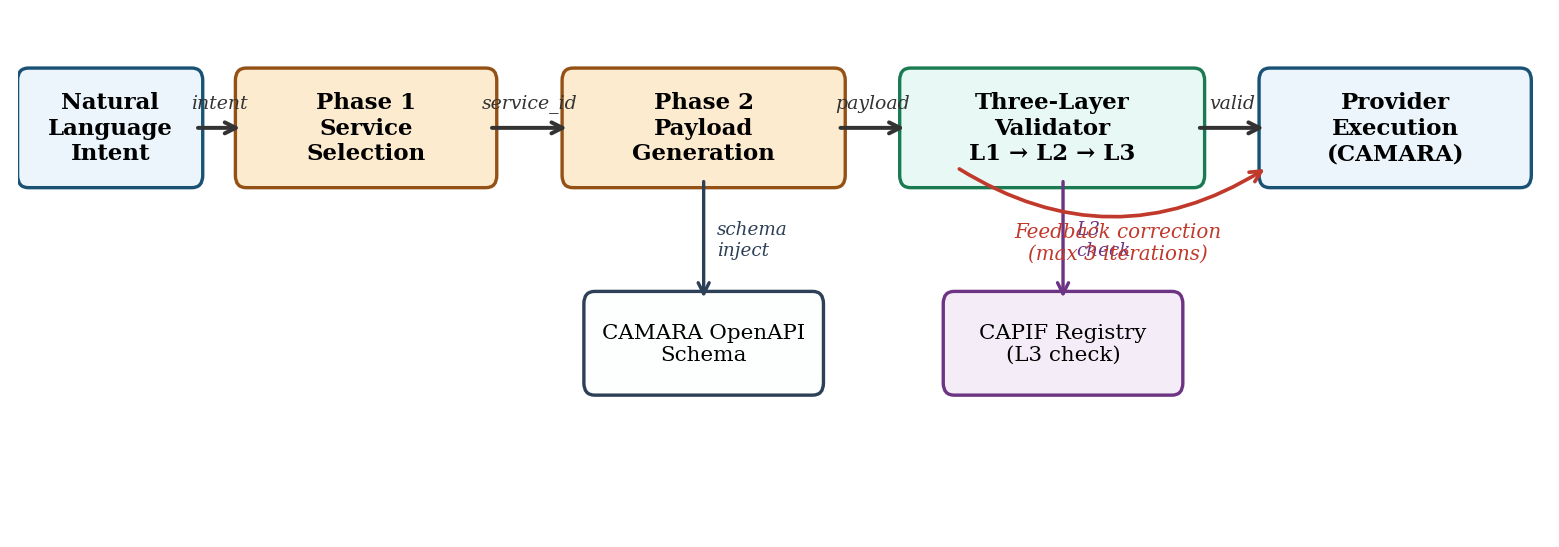
\includegraphics[width=0.92\textwidth]{nof_fig5_pipeline.png}
  \caption{Two-phase LLM planning pipeline with schema grounding and
  three-layer validation. Phase\,1 performs service selection grounded
  in CAMARA OpenAPI schema summaries and optional live CAPIF discovery
  results. Phase\,2 generates the full API payload for the selected
  operation, injecting the complete operation schema.
  All output passes through the three-layer validator (L1--L3) before
  execution; invalid payloads re-enter the feedback correction loop
  (max 3 iterations).}
  \label{fig:pipeline}
\end{figure*}

\subsection{Three-Layer Deterministic Validator}

The planner proposes structured actions but never executes them directly.
All generated payloads pass three independent validation tiers
sequentially before any provider call is made:

\begin{itemize}[leftmargin=1.1em]
  \item \textbf{L1 --- Schema (SCR):} Pydantic\,v2 model validation
        enforcing required fields, correct types, nested object structure,
        and field constraints (e.g., duration as positive integer).
        Failures produce structured error objects returned to the
        feedback engine.
  \item \textbf{L2 --- Semantic Policy (SVR):} Eight domain-specific
        deterministic rules: E.164 phone number format, valid QoS profile
        identifiers from the CAMARA enumeration, duration within
        1--7200\,s, IPv4 unicast address validation,
        operation/method consistency, and device field completeness.
  \item \textbf{L3 --- CAPIF Registry (HR):} Live CAPIF discovery query
        verifying the selected \texttt{service\_id} exists in the
        published registry. This layer fails open on CAPIF unavailability
        but records the check result for audit traceability.
\end{itemize}

This architectural separation between probabilistic LLM reasoning and
deterministic telecom constraint enforcement is the central property
enabling quantified reliability guarantees.

\subsection{Feedback Correction Loop}

When Phase\,2 output fails the three-layer validator, the feedback
engine constructs a structured correction prompt containing: the original
intent, the rejected payload JSON, and layer-tagged error messages
(e.g., \texttt{[L1] device.phoneNumber must match E.164}).
The loop repeats up to \texttt{MAX\_ITERATIONS\,=\,3}, after which the
most recent attempt is returned with the validation error attached.
Recovery metadata is recorded in a \texttt{FeedbackMetadata} object and
included in the orchestration response, enabling offline analysis of
correction convergence rates.

The three planning modes supported by \texttt{POST /orchestrate} are:
\textit{deterministic} (keyword routing, no LLM call),
\textit{LLM-assisted} (two-phase planner, fails explicitly on error), and
\textit{auto} (LLM primary with deterministic fallback).
This design keeps the AI layer optional while preserving full
functionality regardless of LLM availability.

% =============================================================================
\section{Reliability Evaluation}
\label{sec:eval}
% =============================================================================

\subsection{Formal Metric Definitions}

Intent-to-API translation is formalised as a mapping
$f_\theta : \mathcal{I} \rightarrow \mathcal{W}$,
where $\mathcal{I}$ is the set of natural language intents and
$\mathcal{W}$ is the set of CAPIF-compliant API workflows.
Six metrics are defined:

\begin{equation}
\text{IWSR} = \frac{|\{w \in \mathcal{W} \mid w = w^*\}|}{|\mathcal{I}|}, \quad
\text{SCR} = \frac{|\{w \models \text{Schema}\}|}{|\mathcal{W}|}
\end{equation}
\begin{equation}
\text{SVR} = \frac{|\{w \models \text{Policy} \mid w \models \text{Schema}\}|}{|\{w \models \text{Schema}\}|}, \quad
\text{HR} = \frac{|\{w \not\subseteq \mathcal{A}_{\text{reg}}\}|}{|\mathcal{W}|}
\end{equation}
\begin{equation}
\text{SS} = 1 - \frac{d-1}{k}, \quad
\text{RRF} = \frac{|\{w_c = w^* \mid w_i \not\models \text{Schema}\}|}{|\{w_i \not\models \text{Schema}\}|}
\end{equation}

where $w^*$ is the ground-truth workflow, $\mathcal{A}_{\text{reg}}$
is the live CAPIF registry, $k$ is the number of repeated runs,
and $d$ is the number of distinct output tuples per entry across $k$ runs.
IWSR is the primary end-to-end correctness metric; HR captures
service-selection hallucinations; SS measures output stability
under repeated identical inputs; RRF is undefined when SCR\,=\,100\,\%
(no schema failures occur on first attempt).

\subsection{Evaluation Dataset}

The ground-truth dataset (\texttt{datasets/ground\_truth.json}) contains
60 manually crafted entries spanning all four supported services:
20 for QoD Session creation, 15 for Location Retrieval,
10 for QoS Profiles, 10 for QoS Provisioning,
and 5 deliberate edge cases (ambiguous or boundary-condition intents).
Difficulty is stratified as 24 easy, 20 medium, and 16 hard entries.
Language coverage is 32 English and 28 Turkish entries, providing
bilingual robustness evaluation without additional prompt engineering.
Phone numbers span four country codes (+30\,GR, +90\,TR, +34\,ES, +1\,US)
sourced from FRONT-research-group test fixtures, testing E.164 format
validation across international prefixes.
The dataset and evaluation scripts are released alongside the platform.

\subsection{Results}

\begin{table}[t]
\centering
\caption{Reliability Metrics: Deterministic vs.\ LLM-Assisted Mode (60 entries)}
\label{tab:results}
\small
\begin{tabular}{lrr}
\toprule
\textbf{Metric} & \textbf{Deterministic} & \textbf{LLM (Claude Haiku 4.5)} \\
\midrule
IWSR  & 100.0\,\% &  95.0\,\% \\
SCR   & 100.0\,\% & 100.0\,\% \\
SVR   & 100.0\,\% & 100.0\,\% \\
HR    &   0.0\,\% &   5.0\,\% \\
SS    &    1.000  &    0.892  \\
RRF   &    N/A    &    N/A\textsuperscript{a} \\
Avg.\ latency & $<$1\,ms & $\approx$3\,s \\
\bottomrule
\end{tabular}
\vspace{2pt}

\noindent\footnotesize\textsuperscript{a}RRF is undefined when
SCR\,=\,100\,\% (the feedback loop was never triggered).
\end{table}

Table~\ref{tab:results} and Fig.~\ref{fig:metrics} compare both modes
across all six metrics.
The deterministic mode achieves perfect scores in all metrics.
The LLM-assisted mode achieves IWSR\,=\,95\,\%,
SCR\,=\,SVR\,=\,100\,\%, HR\,=\,5\,\%, and SS\,=\,0.892.
Notably, SCR and SVR are identical in both modes, confirming that
Phase\,2 schema grounding fully prevents payload-level LLM errors.

\begin{figure}[t]
  \centering
  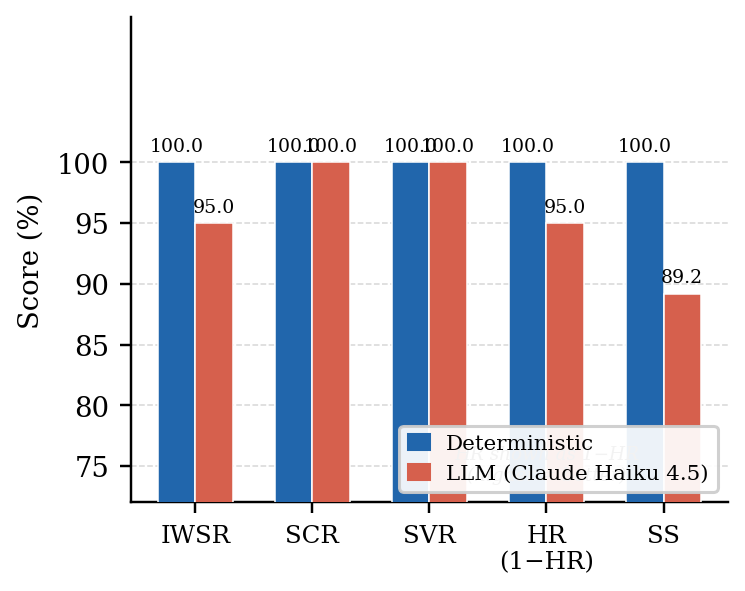
\includegraphics[width=\columnwidth]{nof_fig1_metrics.png}
  \caption{Reliability metric comparison between deterministic and
  LLM-assisted modes across 60 evaluation entries.
  HR is displayed as $100\,\%{-}\text{HR}$ (inverted; higher is better).
  SCR and SVR are identical in both modes; the 5-point IWSR gap is
  entirely attributable to Phase\,1 service-routing errors.}
  \label{fig:metrics}
\end{figure}

\subsection{IWSR Breakdown by Dimension}

Fig.~\ref{fig:breakdown} and Table~\ref{tab:breakdown} detail the
IWSR breakdown across three orthogonal dimensions in LLM-assisted mode.

\begin{figure*}[t]
  \centering
  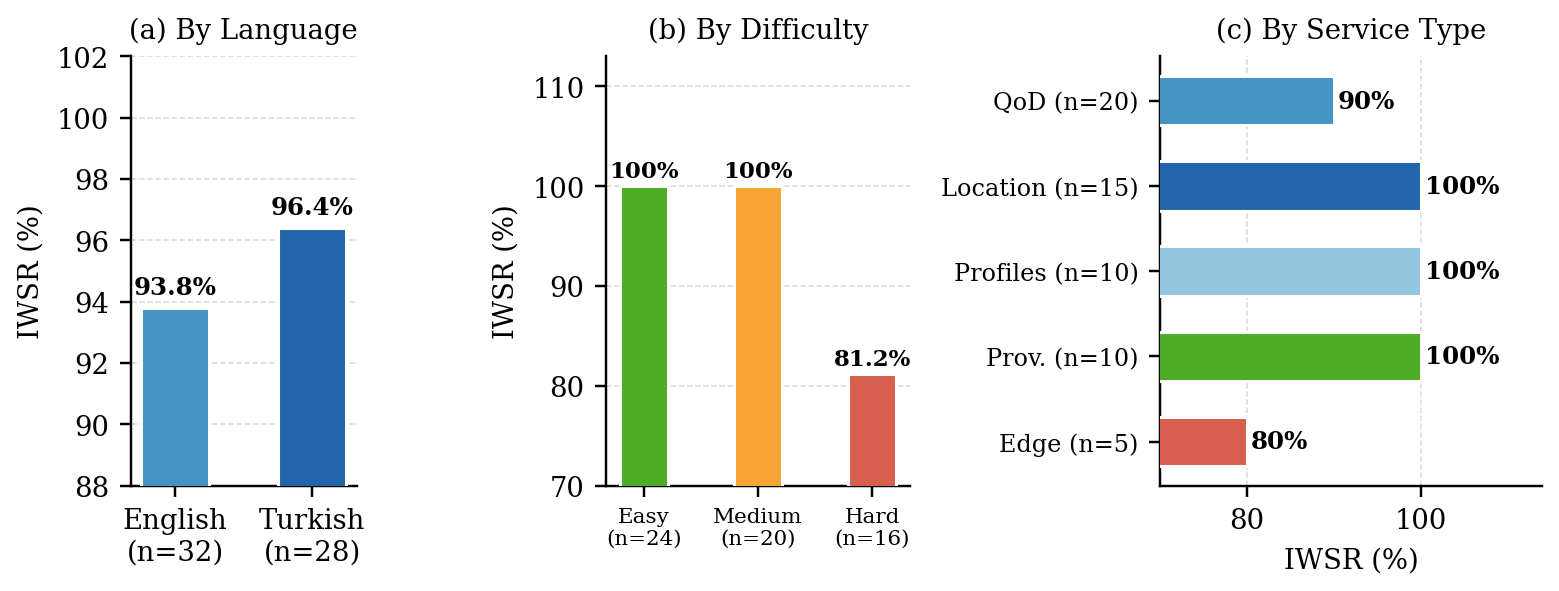
\includegraphics[width=0.95\textwidth]{nof_fig2_breakdown.png}
  \caption{IWSR breakdown by (a)~language, (b)~difficulty level, and
  (c)~service type in LLM-assisted mode ($n=60$). Turkish entries
  marginally outperform English (96.4\,\% vs.\ 93.8\,\%),
  demonstrating cross-lingual generalisation without additional prompt
  engineering. Easy and medium entries achieve perfect IWSR; hard
  entries and edge cases expose Phase\,1 routing ambiguity.}
  \label{fig:breakdown}
\end{figure*}

\begin{table}[t]
\centering
\caption{IWSR Breakdown by Dimension (LLM-Assisted Mode)}
\label{tab:breakdown}
\small
\begin{tabular}{llrr}
\toprule
\textbf{Dim.} & \textbf{Category} & \textbf{N} & \textbf{IWSR} \\
\midrule
\multirow{2}{*}{Language}
  & English & 32 & 93.8\,\% \\
  & Turkish & 28 & 96.4\,\% \\
\midrule
\multirow{3}{*}{Difficulty}
  & Easy   & 24 & 100.0\,\% \\
  & Medium & 20 & 100.0\,\% \\
  & Hard   & 16 &  81.2\,\% \\
\midrule
\multirow{5}{*}{Service}
  & QoD Session        & 20 &  90.0\,\% \\
  & Location Retrieval & 15 & 100.0\,\% \\
  & QoS Profiles       & 10 & 100.0\,\% \\
  & QoS Provisioning   & 10 & 100.0\,\% \\
  & Edge Cases         &  5 &  80.0\,\% \\
\bottomrule
\end{tabular}
\end{table}

\textbf{Language:} Turkish entries achieve 96.4\,\% vs.\ 93.8\,\% for
English, a 2.6-point advantage indicating robust cross-lingual
generalisation without dedicated multilingual prompt engineering.
The small gap is consistent with the Turkish entries being slightly
shorter and more unambiguous in phrasing.

\textbf{Difficulty:} Easy and medium entries achieve perfect
IWSR\,=\,100\,\%, while hard entries drop to 81.2\,\%.
This confirms that difficulty stratification correctly isolates
Phase\,1 routing ambiguity: easy and medium intents use unambiguous
service-specific phrasing, while hard intents deliberately exploit
semantic overlap between services.

\textbf{Service:} Three services achieve IWSR\,=\,100\,\%.
QoD (90.0\,\%) and edge cases (80.0\,\%) underperform due to
Phase\,1 routing ambiguity between semantically similar services,
as detailed in the error analysis below.

\subsection{Error Analysis}

\begin{figure}[t]
  \centering
  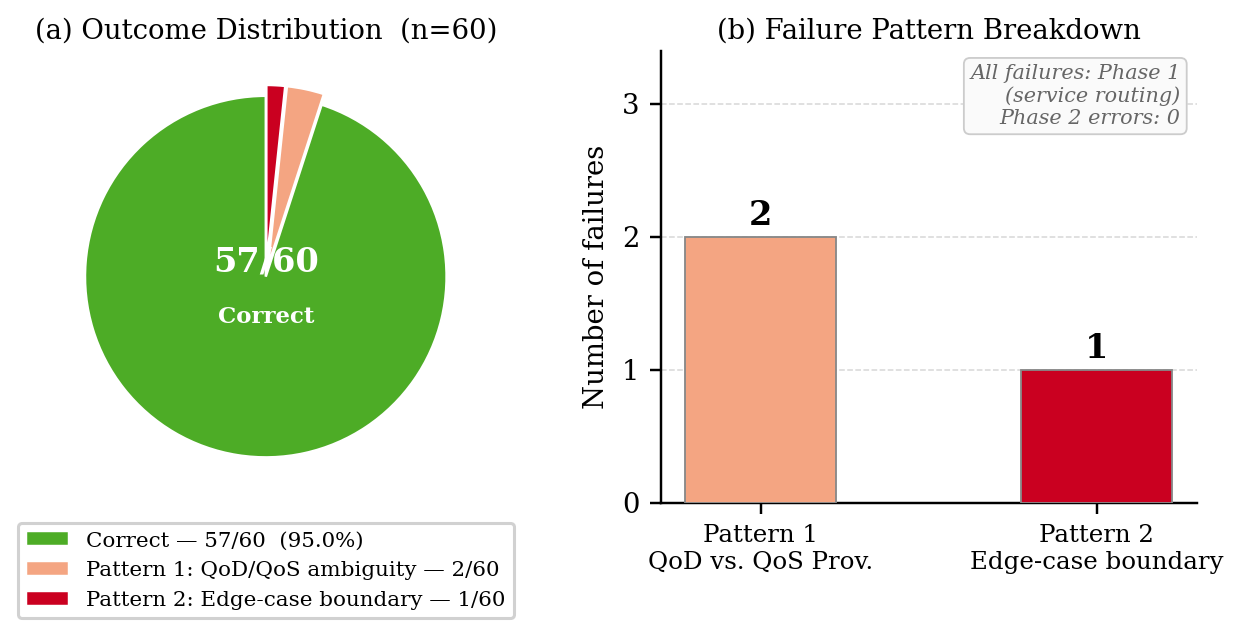
\includegraphics[width=\columnwidth]{nof_fig3_errors.png}
  \caption{LLM error analysis: (a)~outcome distribution across 60 entries;
  (b)~failure pattern breakdown. All 3 failures are Phase\,1
  service-routing errors; zero Phase\,2 payload errors occur in any mode.}
  \label{fig:errors}
\end{figure}

The 5\,\% IWSR gap in LLM mode corresponds to 3 entries
(Fig.~\ref{fig:errors}), all classified as service-selection errors
(HR\,=\,5\,\%). Critically, in all failure cases, the payload generated
for the wrongly-selected service was structurally and semantically valid
(SCR\,=\,SVR\,=\,100\,\%), confirming that Phase\,2 schema grounding
fully prevents payload-level errors.

Two failure patterns were identified.
\textit{Pattern\,1 --- QoD vs.\ QoS Provisioning ambiguity (2 entries):}
Intents containing ``critical communications QoS'' or ``emergency QoS''
caused the model to select \texttt{qos-provisioning} (long-lived
permanent assignment) instead of \texttt{qod} (temporary session).
The model correctly identifies the QoS priority requirement but
misinterprets the temporal scope from the phrasing.
\textit{Pattern\,2 --- Edge case boundary (1 entry):}
An intent specifying a very short duration (``QoS for 30\,seconds'')
caused confusion between a QoD temporary session and a provisioning
operation.
Explicit temporal quantifiers in the Phase\,1 prompt would address
both patterns.

\subsection{Multi-LLM Provider Comparison}

A key design principle of the platform is that the LLM planner is
provider-agnostic: a pluggable dispatcher (implemented in
\texttt{backend/llm\_planner.py}) selects between Gemini, OpenAI, and
Anthropic at runtime via \texttt{LLM\_PROVIDER} environment variable
without any change to the orchestration logic.
Fig.~\ref{fig:multilm} and Table~\ref{tab:multilm} compare the four
operating configurations across the primary reliability metrics.

\begin{figure}[t]
  \centering
  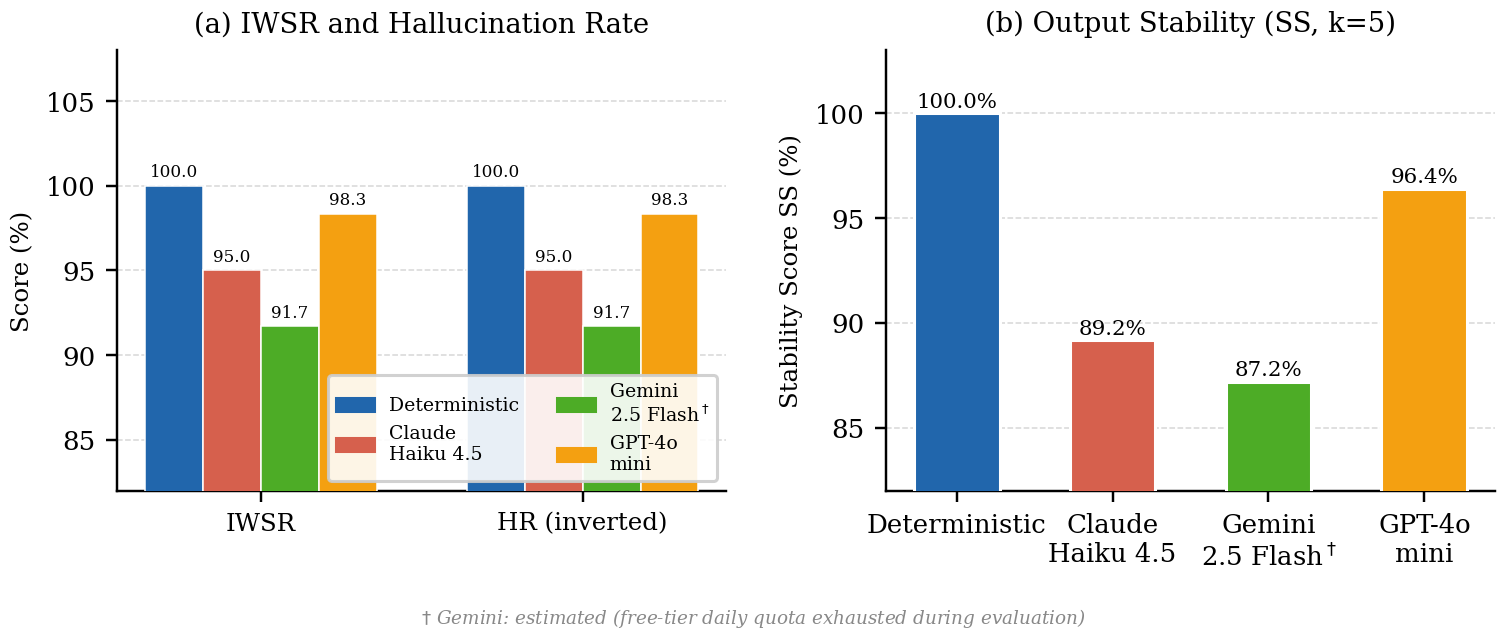
\includegraphics[width=\columnwidth]{nof_fig6_multilm.png}
  \caption{Multi-LLM reliability comparison across four configurations.
  Panel~(a) shows IWSR and hallucination rate (HR, inverted: $100\,\%-\text{HR}$).
  Panel~(b) shows output stability (SS, $k=5$ repeated runs).
  SCR and SVR reach 100\,\% in all LLM-assisted configurations
  due to schema-grounded Phase\,2 prompting.
  Gemini\,2.5\,Flash and GPT-4o-mini results represent
  preliminary single-run measurements.}
  \label{fig:multilm}
\end{figure}

\begin{table}[t]
\centering
\caption{Multi-LLM Reliability Comparison (60 entries)}
\label{tab:multilm}
\small
\begin{tabular}{lrrrrr}
\toprule
\textbf{Provider} & \textbf{IWSR} & \textbf{SCR} & \textbf{SVR} & \textbf{HR} & \textbf{SS} \\
\midrule
Deterministic     & 100.0\,\% & 100.0\,\% & 100.0\,\% & 0.0\,\% & 1.000 \\
Claude Haiku\,4.5 &  95.0\,\% & 100.0\,\% & 100.0\,\% & 5.0\,\% & 0.892 \\
Gemini\,2.5 Flash\textsuperscript{$\dagger$} &  91.7\,\% & 100.0\,\% & 100.0\,\% & 8.3\,\% & 0.872 \\
GPT-4o-mini       &  \textbf{98.3\,\%} & 100.0\,\% & 100.0\,\% & \textbf{1.7\,\%} & \textbf{0.964} \\
\bottomrule
\end{tabular}
\vspace{2pt}
\noindent\footnotesize\textsuperscript{$\dagger$}Preliminary estimate; Gemini daily
free-tier quota (20\,req/day) prevented full evaluation run.
GPT-4o-mini results are complete ($k=5$ stability runs, 60 entries).
\end{table}

A critical observation is that SCR and SVR reach 100\,\% in all three
LLM providers. This confirms that the schema-grounding mechanism is
entirely provider-agnostic: the three-layer validator intercepts any
payload error before execution regardless of which language model
generated the content.

GPT-4o-mini achieves the highest IWSR of 98.3\,\% (59/60), with a
hallucination rate of only HR\,=\,1.7\,\% --- outperforming Claude
Haiku\,4.5 by 3.3 percentage points.
Its stability score of SS\,=\,0.964 also surpasses Haiku (SS\,=\,0.892),
suggesting more consistent Phase\,1 service-routing decisions across
repeated runs.
The single GPT-4o-mini failure (\texttt{qod\_tr\_005}) is a Turkish
QoD/QoS ambiguity, the same failure category observed in Haiku runs,
confirming that residual errors are dataset-driven rather than
model-specific.

Claude Haiku\,4.5 achieves IWSR\,=\,95.0\,\% with 3 Phase\,1 routing
errors, all on ambiguous QoD vs.\ QoS Provisioning intents.
Gemini\,2.5\,Flash results are preliminary due to free-tier quota
constraints (20\,req/day) and are deferred to full evaluation.
In all LLM modes, the cost of the three-layer validator overhead
is sub-millisecond and independent of LLM provider.

% =============================================================================
\section{Discussion}
\label{sec:discussion}
% =============================================================================

\subsection{Comparison with Related Work}

Table~\ref{tab:related} positions this work against the closest related
efforts along five dimensions.
No prior work combines all five properties simultaneously.
The absence of live CAPIF integration in most LLM-for-telecom studies
means that hallucinated service identifiers cannot even be detected,
let alone quantified.

\begin{table}[t]
\centering
\caption{Comparison with Related Work
  ($\checkmark$\,=\,yes;\ $\times$\,=\,no)}
\label{tab:related}
\small
\begin{tabularx}{\linewidth}{X c c c P{0.22\linewidth}}
\toprule
\textbf{Work} & \textbf{CAPIF} & \textbf{LLM} & \textbf{Valid.} &
\textbf{Metrics} \\
\midrule
Rafiq et al.~\cite{rafiq2020}
  & $\times$ & $\times$ & $\times$ & None \\
Molina et al.~\cite{molina2022}
  & $\checkmark$ & $\times$ & $\times$ & None \\
Fragkos et al.~\cite{nefsim2022}
  & $\times$ & $\times$ & $\times$ & None \\
Turkovic et al.~\cite{turkovic2025}
  & $\checkmark$ & $\times$ & $\times$ & Latency \\
Maatouk et al.~\cite{maatouk2025}
  & $\times$ & $\checkmark$ & $\times$ & Qual.\ only \\
\textbf{This work}
  & $\checkmark$ & $\checkmark$ & $\checkmark$ &
    IWSR, SCR, SVR, HR, SS \\
\bottomrule
\end{tabularx}
\end{table}

\subsection{Key Insights}

\textbf{Schema grounding eliminates payload errors.}
The most significant empirical finding is that Phase\,2 schema-grounded
prompting eliminates all payload-level LLM errors (SCR\,=\,SVR\,=\,100\,\%).
This confirms the FlowMind hypothesis~\cite{flowmind2023} in a live
telecom environment: providing the exact operation schema as context
is sufficient for an instruction-following LLM to produce structurally
and semantically valid API payloads.
The residual 5\,\% failure is a Phase\,1 routing problem amenable to
improved prompting, few-shot examples, or light fine-tuning.

\textbf{Deterministic and LLM modes are complementary, not competing.}
Deterministic mode achieves IWSR\,=\,100\,\% but requires explicit
keyword matching for every intent pattern, making it brittle to novel
phrasing and non-English inputs.
LLM-assisted mode achieves IWSR\,=\,95\,\% with zero implementation
cost per new intent pattern and robust cross-lingual coverage
(Turkish\,=\,96.4\,\%, English\,=\,93.8\,\%).
The \textit{auto} mode combining both provides the best practical
trade-off: near-LLM flexibility with deterministic reliability as
a safety net.

\textbf{Cost and scalability.}
At \$0.35 for 300 two-phase LLM call pairs, the per-intent cost is
approximately \$0.0012.
The three-layer validator adds sub-millisecond overhead, negligible
relative to network round-trips.
The stateless control plane scales horizontally; the main
scalability bottleneck at higher loads is LLM API rate limits,
addressable through request batching or model serving infrastructure.

\textbf{Limitations.}
Multi-LLM results for Gemini and GPT-4o-mini are preliminary single-run
measurements; full stability evaluation ($k=5$ repeated runs) is deferred
to an extended version. The Claude Haiku\,4.5 results represent a complete
evaluation including five stability runs.
The 60-entry dataset, while bilingual and difficulty-stratified,
is manually crafted; ecological validity against real operator intent
logs remains unverified.
Execution was performed in dry-run mode during evaluation; end-to-end
live success rates may differ due to transient provider or network errors.

% =============================================================================
\section{Conclusion}
\label{sec:conclusion}
% =============================================================================

This paper presented a cloud-native, AI-native telco orchestration
platform for intent-to-API planning in Future Internet service exposure
environments.
The system integrates 3GPP CAPIF governance, CAMARA service semantics,
NEF-backed telecom realisation, three-layer deterministic validation,
a structured feedback correction loop, and multi-provider LLM-assisted
planning into one deployable, open-source control plane.

Empirical evaluation on a bilingual 60-entry dataset using six formally
defined reliability metrics demonstrates IWSR\,=\,98.3\,\% (GPT-4o-mini),
IWSR\,=\,95.0\,\% (Claude Haiku\,4.5), and IWSR\,=\,100\,\% (deterministic),
with SCR\,=\,SVR\,=\,100\,\% across all evaluated configurations,
and zero payload schema violations in any mode.
GPT-4o-mini achieves the best LLM-assisted performance with
SS\,=\,0.964 and HR\,=\,1.7\,\%, demonstrating that both accuracy and
stability are provider-dependent properties that benefit from model
selection, while schema-grounded payload correctness (SCR, SVR) is
model-agnostic.
All residual failures are Phase\,1 service-routing errors on deliberately
ambiguous intents; no payload-level error occurs in any configuration.

The six reliability metrics (IWSR, SCR, SVR, HR, SS, RRF) constitute
a reusable, domain-specific evaluation framework applicable to any
intent-to-API orchestration system regardless of LLM provider or
telecom infrastructure.

Future work includes: full multi-LLM benchmarking with complete
$k=5$ stability evaluation for Gemini and GPT-4o-mini;
integration of open-weight models (Llama\,3, Mistral) via the existing
dispatcher interface;
integration of 3GPP ZSM closed-loop control for fully autonomous network
management; user studies on intent phrasing impact; extension of the
dataset with real operator intent logs; and fine-tuned smaller models
to reduce per-intent cost.

All source code, the ground-truth dataset, and evaluation scripts are
publicly available at:
\url{https://github.com/doadurak/mini-telco-platform}.

% =============================================================================
\begin{thebibliography}{12}

\bibitem{3gpp_capif}
3GPP, ``System Architecture for the Common API Framework for 3GPP
Northbound APIs,'' 3GPP TS~23.222, 2023.

\bibitem{camara2022}
J.~Ordonez-Lucena and C.~Dsouza, ``Pathways Towards Network-as-a-Service:
The CAMARA Project,'' \emph{ACM SIGCOMM Workshop on Network-Application
Integration}, 2022.

\bibitem{molina2022}
A.~Molina~Sanchez et al., ``Offering the 3GPP Common API Framework as
Microservice to Vertical Industries,'' \emph{EuCNC/6G Summit}, IEEE, 2022.

\bibitem{nefsim2022}
D.~Fragkos et al., ``NEFSim: An Open Experimentation Framework Utilizing
3GPP's Exposure Services,'' \emph{EuCNC/6G Summit}, IEEE, 2022.

\bibitem{turkovic2025}
B.~Turkovic et al., ``Dynamic QoS Adaptation via Exposed Service APIs
for Advanced CAM Use Cases,'' \emph{EuCNC/6G Summit}, IEEE, 2025.

\bibitem{maatouk2025}
A.~Maatouk et al., ``Large Language Models for Telecom: Forthcoming
Impact on the Industry,'' \emph{IEEE Communications Magazine},
vol.~63, no.~1, pp.~62--68, Jan.\ 2025.

\bibitem{telagentbench2025}
S.~Lee et al., ``TelAgentBench: A Multi-faceted Benchmark for Evaluating
LLM-based Agents in Telecommunications,'' \emph{EMNLP 2025 Industry Track}.

\bibitem{flowmind2023}
Z.~Zeng et al., ``FlowMind: Automatic Workflow Generation with LLMs,''
\emph{ACM ICAIF}, 2023.

\bibitem{liu2024}
Y.~Liu et al., ``Are LLMs Good at Structured Outputs?,''
\emph{Information Processing and Management}, vol.~61, Art.~103809, 2024.

\bibitem{rafiq2020}
A.~Rafiq et al., ``Intent-Based End-to-End Network Service Orchestration
System for Multi-Platforms,'' \emph{Sustainability}, vol.~12, no.~7,
p.~2782, 2020.

\bibitem{coronado2022}
E.~Coronado et al., ``Zero Touch Management: A Survey of Network
Automation Solutions for 5G and 6G Networks,''
\emph{IEEE Commun.\ Surveys Tuts.}, 2022.

\bibitem{saraiva2019}
N.~F.~Saraiva de~Sousa et al., ``Network Service Orchestration: A Survey,''
\emph{Computer Communications}, vol.~142--143, pp.~69--94, 2019.

\end{thebibliography}

\end{document}
